%! TEX root = course_report.tex

\section{Платформа Android}
\label{sec:android_platform}

ОС Android появилась более 15 лет назад.
Вскоре после этого права на ОС купила корпорация Google, увидев в ней огромный потенциал.
В результате на сегодняшний день Android -- самая популярная ОС для мобильных устройств с рыночной долей в 71\%, по данным StatCounter \cite{statcounter_mobile_os}.
StatCounter~-- сервис веб-аналитики, установленный на более чем 2 миллионах сайтов по всему миру.
Отчёты StatCounter основываются на данных веб-аналитики \cite{statcounter_methodology}.

Говоря об Android, обычно подразумевают платформу Android -- более широкое понятие, включающее в себя, помимо слоя абстракции оборудования (англ. \textit{Hardware Abstraction Layer}) и ядра, различные высокоуровневые средства для создания пользовательских приложений на языках Java и Kotlin.

\subsection{Структура и архитектура платформы}
\label{sub:android_platform:struct_and_arch}

Платформа Android состоит из нескольких слоёв абстракции, разделённых между собой для упрощения разработки каждого из них.
Далее будет рассмотрен каждый из этих слоёв.

\subsubsection{}
\label{subsub:android_platform:struct_and_arch:linux}
\textit{Ядро Linux} лежит в основе платформы Android.
Одна из причин использования ядра Linux -- широкие возможности Linux, нацеленные на повышение безопасности \cite{android_kernel_security}:
\begin{itemize}
	\item безопасное межпроцессное взаимодействие;
	\item изоляция приложений друг от друга;
	\item система прав доступа к файлам и папкам;
	\item защита загрузчика от несанкционированного изменения;
	\item современные криптографические алгоритмы.
\end{itemize}
Вместе со сборкой ядра Linux производители мобильных устройств поставляют драйверы оборудования (обычно в виде модулей с закрытым исходным кодом).

\subsubsection{}
\label{subsub:android_platform:struct_and_arch:hal}
\textit{Слой абстракции оборудования (HAL)} работает поверх ядра.
Он содержит библиотеки функций для более удобного доступа к оборудованию различных производителей из вышестоящих уровней абстракции.
HAL состоит из нескольких модулей, каждый из которых реализует интерфейс для определённого типа оборудования: камера, Bluetooth-модуль, микрофон, звуковой динамик и т. д. 

\subsubsection{}
\label{subsub:android_platform:struct_and_arch:art}
\textit{Android Runtime (ART)} -- среда выполнения Java и Kotlin приложений.
Она осуществляет компиляцию байт-кода ART в машинный код процессора, установленного в пользовательском устройстве.
ART пришла на cмену Dalvik в версии Android 5.0.
Одним из преимуществ ART по сравнению с Dalvik является компиляция приложений во время установки в машинный код устройства (англ. \textit{ahead-of-time}).
Это позволяет сократить время запуска приложения.
При этом установка приложений может занимать больше времени, чем при компиляции во время выполнения (англ. \textit{just-in-time}).

На одном уровне с \textit{ART} находятся \textit{системные C и C++ библиотеки}, предоставляющие высокоуровневый интерфейс для распространённых задач:
\begin{itemize}
	\item отображениe веб-страниц (Android System WebView);
	\item стандартная библиотека языка C (Bionic);
	\item работа с графикой (OpenGL ES и Vulkan);
	\item работа со звуком (OpenSL ES) и др.
\end{itemize}

При разработке приложений с использованием Android NDK возможно напрямую работать с вышеописанными библиотеками.

\subsubsection{}
\label{subsub:android_platform:struct_and_arch:java_api}
\textit{Java API Framework} оборачивает \textit{системные библиотеки} и \textit{слой абстракции оборудования} в Java-классы, которые используются в системных и пользовательских приложениях. В состав Java API Framework входят:
\begin{itemize}
	\item \textit{View System} -- расширяемая система компонентов пользовательского интерфейса (кнопки, списки, поля ввода текста и т. д.);
	\item \textit{Resource Manager} -- управление файлами локализации, графики и описания пользовательского интерфейса;
	\item \textit{Notification Manager} -- для отображения оповещений в строке состояния (т. н. <<шторка>>);
	\item \textit{Activity Manager}, управляющий жизненным циклом приложения и навигацией между экранами;
	\item \textit{Content Providers}, служащие для доступа к данным из других приложений (например, к списку контактов) и др.
\end{itemize}

\subsubsection{}
\label{subsub:android_platform:struct_and_arch:system_apps}
\textit{Стандартные системные приложения} составляют самый высокий уровень абстракции и включают:
\begin{itemize}
	\item приложение для совершения звонков по мобильной сети (\textit{Dialer});
	\item приложение для отправки SMS;
	\item клиент электронной почты;
	\item камера и др.
\end{itemize}

На рисунке~\ref{fig:android_platform_arch} представлены компоненты платформы Android \cite{android_platform_arch}.

\begin{figure}[p]
    \centering
    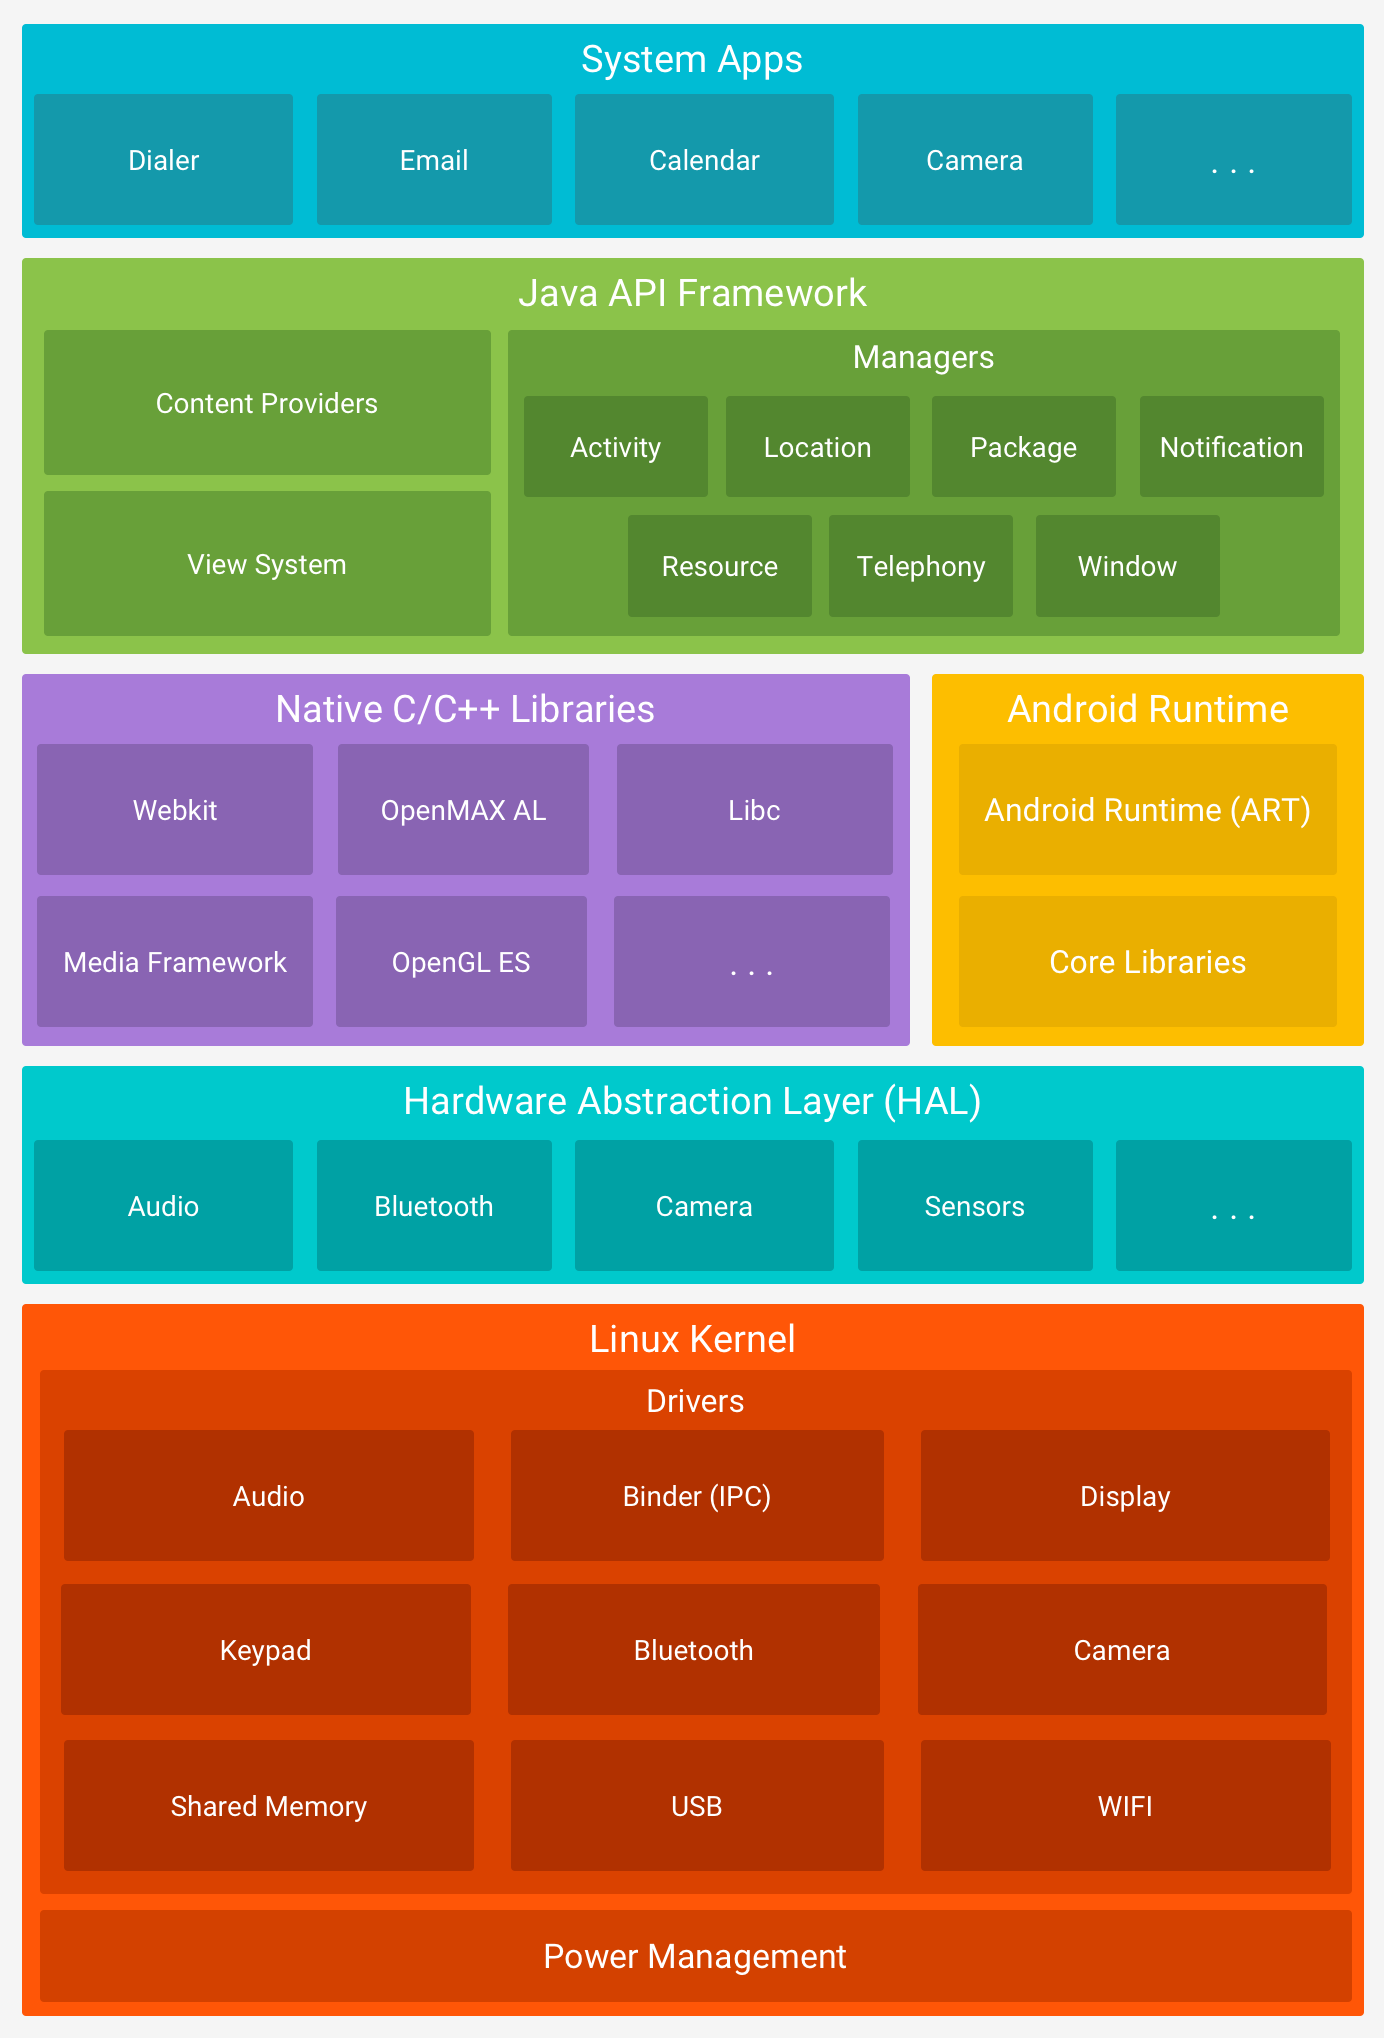
\includegraphics[width=1.0\textwidth]{android_platform_arch.png}  
    \caption{Компоненты платформы Android}
	\label{fig:android_platform_arch}
\end{figure}

\subsection{История версий Android}
\label{sub:android_platform:history}

\subsection{Сравнение Android с другими мобильными платформами}
\label{sub:android_platform:comparison}

\subsubsection{Преимущества Android}
\label{subsub:android_platform:comparison:pros}

\subsubsection{Недостатки Android}
\label{suubsub:android_platform:comparison:cons}
